\chapter{Simulations}
\label{simulations}

In order to test and validate the different algorithms proposed in chapter \ref{algos}, a simulation was implemented. The advantages of such simulations is to get rid of the technical constraints of electronic materials, no configuration of the antennas was needed, no need to implement features in the application to deal with the \gls{cir}, no need to modify the state machines presented in appendix \ref{app:state_machine}, etc.
\vspace{2mm}

However, this simulation needs to be as true as possible compared to the reality. This implementation is detailed in the first section of this chapter. Then, the results obtains using this simulation are presented in the following sections for the locating methods presented in \ref{algos}.

\section{Simulation}

The simulation has been created by adapting a code previously developed for the project of the course of Communication Channel given at the ULB \cite{dedoncker2019course}. This simulation is based on the ray tracing, a rendering technique used to compute the trajectory of electro-magnetic waves presented in section \ref{ray_tracing}. Two important features of this program can be separated. The first objective being to simulated a realistic \gls{cir} similar to the one produced by the experimental set-up. The second objective is to perform the localization based on this realistic \gls{cir}.
\vspace{2mm}

\subsection{Realistic CIR generation}

To achieve this objective, first the desired environment has to be simulated in the program. To make it happen, the $\texttt{room\_configuration.m}$ file has been created. Configuration of the geometry of the room, the type of walls used, the number of different furniture and their location in the room can also be chosen. This file is also used to chose the location of the anchor and the tag in the room. The left figure of the Fig. \ref{fig:peaks_real} has been produced using this configuration file.
\vspace{2mm}

In order to generate a finite-band \gls{cir}, the equivalent infinite-band \gls{cir} is first generated. This is can be done for a direct ray, simple reflected ray, double reflected ray and triple reflected ray the transmission across the different materials is also taken into account. The ray reflected on the ground is also computed but not represented for the sake of clarity. An example of all the other ray can be found in Fig. \ref{fig:ray_simu}. On this figure, furnitures are displayed against the walls, the direct ray is displayed in red, a simple reflected ray on one of the furniture in blue, a double reflected ray in cyan and a triple reflection ray is displayed in green.

\begin{figure}[H]
\centering
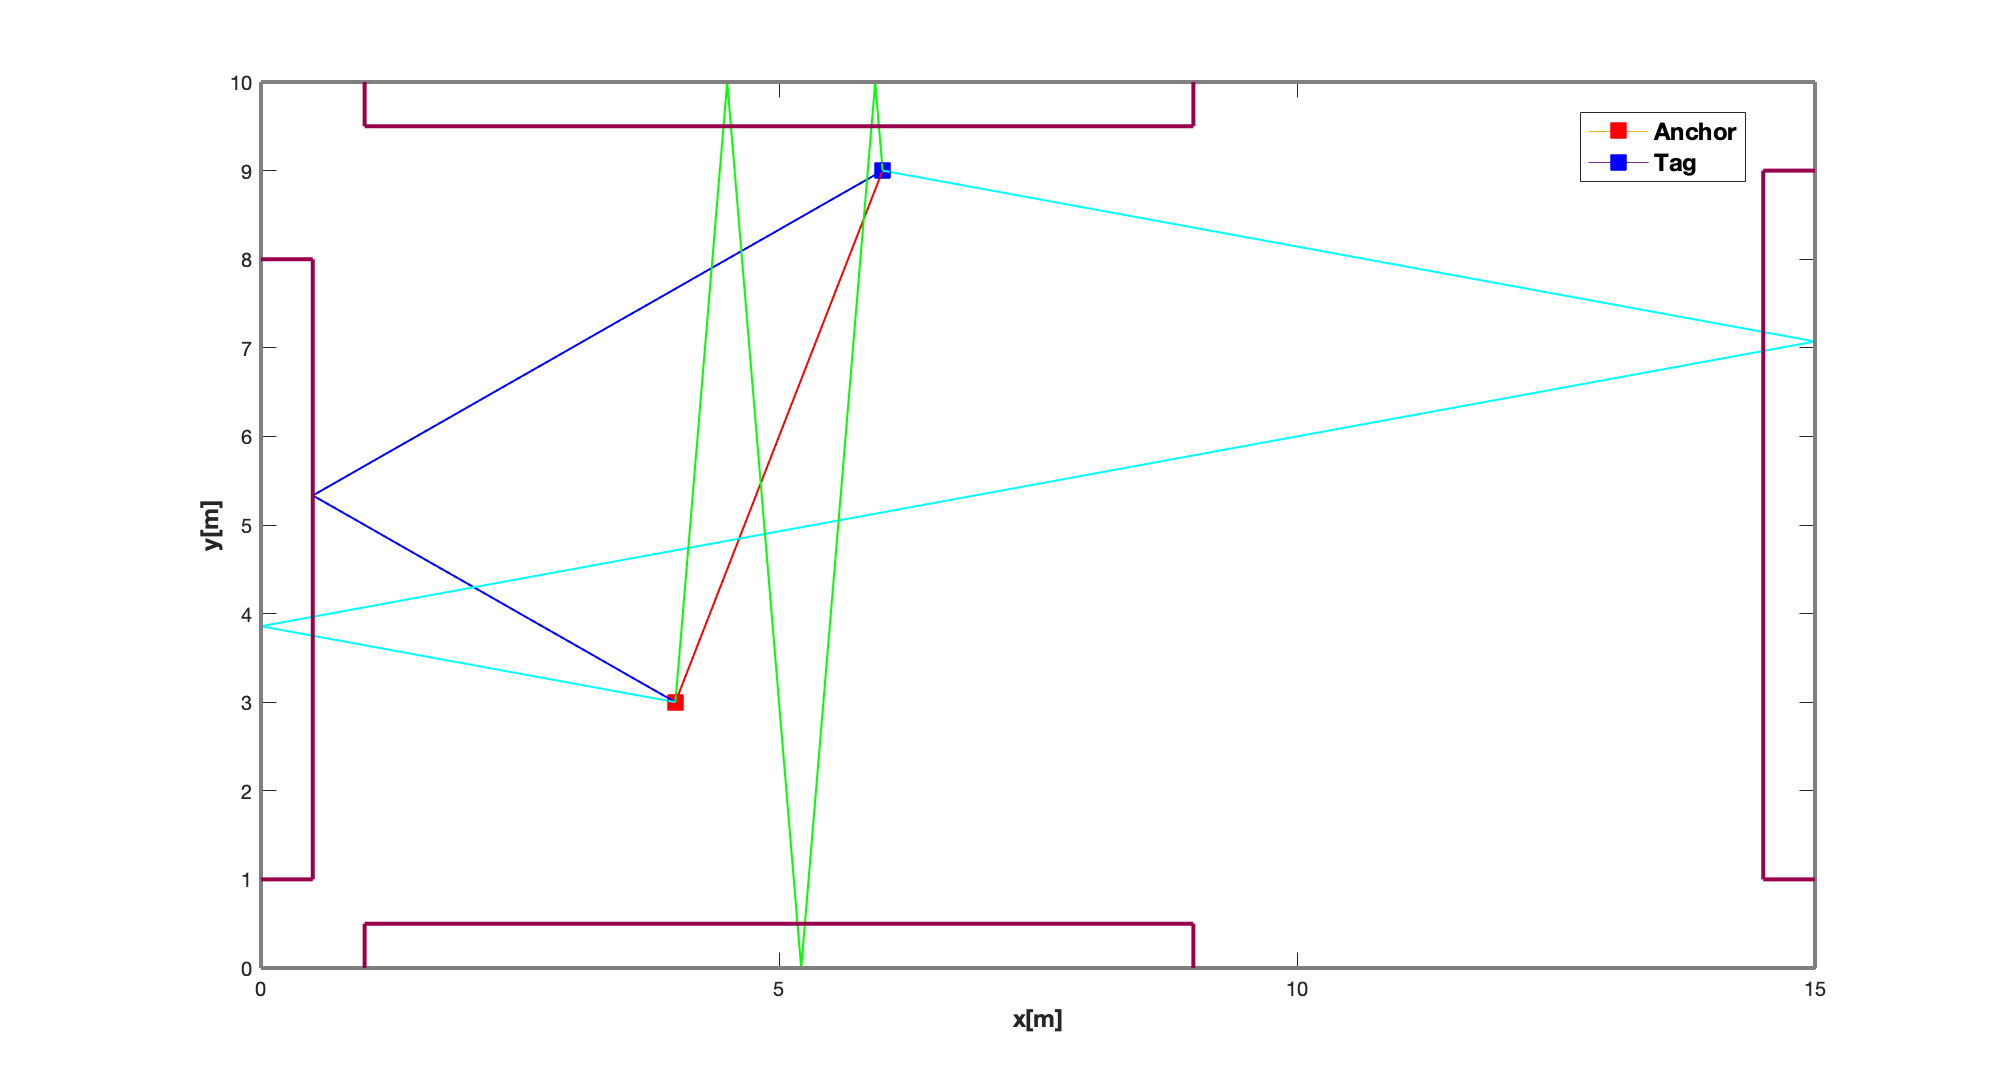
\includegraphics[width=.75\linewidth]{Images/rays_example.png}
\caption{Ray Tracing Simulation - Example. \label{fig:ray_simu}}
\end{figure}

Stating infinite is not completely correct, the real bandwidth being the one of the career frequency in this case, however, in presents the characteristics in regard to actual bandwidth used. The different peaks well isolated and punctual. The so-called infinite-band \gls{cir} is converted to the frequency domain using the Fourier transform. The built-in \gls{fft} function from $\text{MATLAB}$ has been used \cite{mathworks}. The frequency spectrum has been reduced from the carrier frequency to $\text{500 MHz}$, an approximation of the bandwidth used as detailed in section \ref{dwm1000}. Applying the \gls{ifft} to return into the time domain results in the red curve on Fig. \ref{fig:conv_fin}.

\begin{figure}[H]
\centering
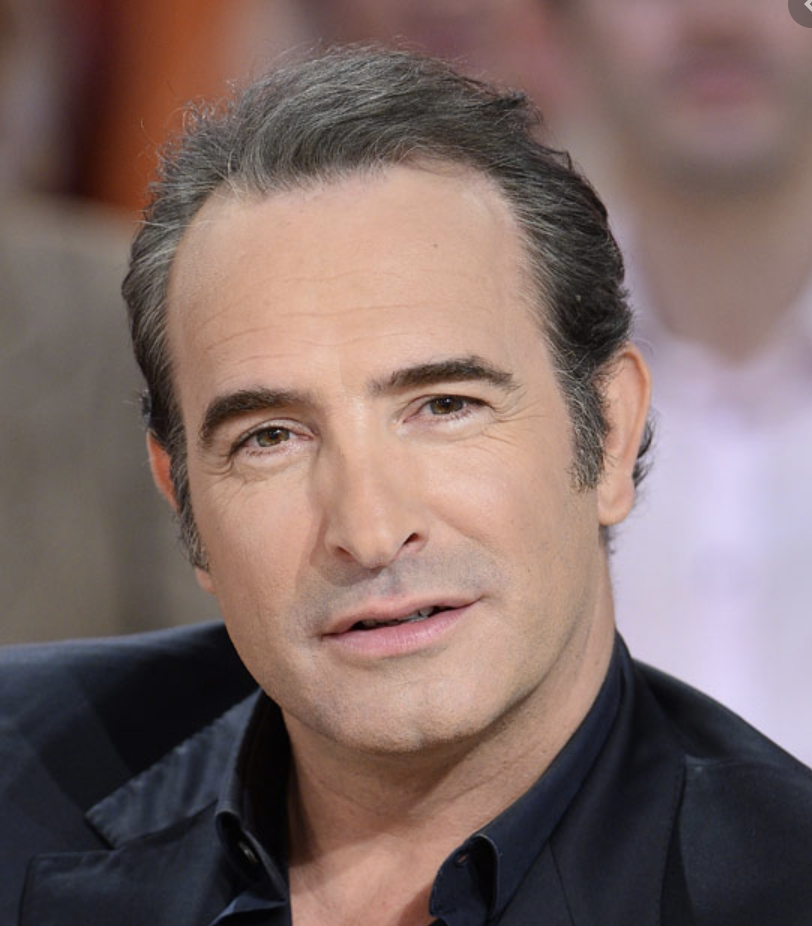
\includegraphics[width=.2\linewidth]{Images/Temporary_pic.png}
\caption{Trouver un nom \label{fig:conv_fin}}
\end{figure}

As one can observe, this \gls{cir} is far from ideal, mostly due to the sides lobes appearing next to every peaks. This is a side effect due to the reduction of the bandwidth. In order to counter this effect, a Chebyshev window has been used \cite{lynch1997dolph}, \cite{mathworks}. The convolution of the finite-band time domain \gls{cir} will reduces those side lobes. The orange curve from Fig. \ref{fig:conv_fin} has been produced using a the $\text{chebyshev}$ function from MATLAB. The parameter of the Chebyshev window has been set heuristically to 25. A systematic method would have been to use an experimental and a simulated \gls{cir} that would correspond to the same situation\footnote{The same room, antennas configuration, antennas position, ...}. The optimal parameter would then be computed using the $\text{lsqcurvefit}$ function from MATLAB.

\subsection{Code possible outputs ?}

The second objective of the simulation is the locating process. As detailed in the chapter \ref{algos}, two different method have been implemented in this scope. In order to compare both methods, JE NE SAIS PAS TROP QUOI DIRE BLABLABLABLABLA....

\section{Hard Simulation}


\section{Soft Simulation}
